\documentclass[loesung]{schulein}
%
\kopfDatum{\today} 
\fach{in-Z1}
\dokName{MOPS}
\keineSeitenzahlen
\usepackage[utf8]{inputenc}
\usepackage{lmodern}
\usepackage{graphicx}
\usepackage{setspace}
\usepackage{environ}
\usepackage{lipsum}
\usepackage{tabularx}
\usepackage[a4paper]{geometry} 
\geometry{top=25mm,left=25mm ,right=25mm, bottom=3cm} 
%
% =======================
% Abbildungstext anpassen
% =======================
\usepackage[normal,font={small}, labelfont=bf,figurename=Abb.]{caption}
%
% Pfad der Abbildungen
\graphicspath{ {../figures/} }
%
\setlength{\footheight}{50mm}
\ifoot{\footnotesize  Letzte Änderung: \today}
\ofoot{Seite Nr. \luecke{1cm}}
\ohead{Datum:\hspace*{3cm}}
%
% ----------
% ÜBERSHRIFT
% ----------
\newcommand{\Ueberschrift}[2]{
	\vskip 1.em
	\setlength{\tabcolsep}{0mm} % kein Innenrand bei Spaleten
	\begin{tabularx}{\linewidth}{lXr}
	{\Large\textbf{\textsf{#1}}} & &
	\includegraphics[height=1.5cm]{#2}\\ % Logo rechtsbündig
	\hline
	\end{tabularx}
	% Spaltenabstand zurücksetzen
	\setlength{\tabcolsep}{6pt} 
}
% ----------
% HINWEISBOX
% ----------
\NewEnviron{hinweisbox}[2]{%
\par
\vspace{1em}
\noindent
\begin{tikzpicture}[]
	\node[rectangle,minimum width=1.0\textwidth, inner sep=0pt] (m) {
		\begin{minipage}{\textwidth}
			\dimen0\linewidth
			\advance\dimen0 by -3.0em
    			\vskip .8em \hspace{1em}
    			\parbox{\the\dimen0}{
        			\BODY\vskip .5em}%			
		\end{minipage}
		};
	\draw[#2, very thick, rounded corners, color=#1] (m.south west) rectangle (m.north east);
\end{tikzpicture}
}
% ----------
% MERKE
% ----------
\NewEnviron{merke}{%
\par
\vspace{1em}
\noindent
\begin{tikzpicture}
	\node[rectangle,minimum width=1.0\textwidth, inner sep=0pt] (m) {
		\begin{minipage}{\textwidth}
			\dimen0\linewidth
			\advance\dimen0 by -3.0em
    			\vskip .8em \hspace{1em}
    			\parbox{\the\dimen0}{
        		\textbf{Merke:}	\BODY\vskip .5em}%			
		\end{minipage}
		};
	\draw[dotted, very thick, rounded corners, color=red] (m.south west) rectangle (m.north east);
\end{tikzpicture}
}
%
\newcommand{\Quelle}[1]{
	\ifoot{\footnotesize #1 \newline Letzte Änderung: \today }
}
%
% ----------
% Schwierigkeitsindikatoren
% ----------
\newcommand{\indikator}[1]{
	\begin{tikzpicture}[]
		\draw[green!50!black] circle (1.5mm);	
		\filldraw[fill=green!20!white, draw=green!50!black]
		(0,0) -- (1.5mm,0mm) arc (0: #1 :1.5mm) -- (0,0);	
	\end{tikzpicture}
}
%
\newcommand{\schwer}{
\begin{tikzpicture}[]
	\filldraw[fill=green!20!white, draw=green!50!black] (0,0) circle (1.5mm);
\end{tikzpicture}
}
\newcommand{\mittel}{
	\indikator{180}
}
\newcommand{\leicht}{
\begin{tikzpicture}[]
	\draw[green!50!black] (0,0) circle (1.5mm);
\end{tikzpicture}
}
% ----------
% AUFGABENBOX
% ----------
\NewEnviron{aufgabenbox}[2]{%
\par
\vspace{1em}
\noindent
\begin{tikzpicture}[]
	\node[rectangle,minimum width=1.0\textwidth, inner sep=0pt] (m) {
		\begin{minipage}{\textwidth}
			\dimen0\linewidth
			\advance\dimen0 by -3.0em
    			\vskip .8em \hspace{1em}
    			\parbox{\the\dimen0}{
        			\BODY\vskip .5em}%			
		\end{minipage}
		};
	\draw[solid, thin, color=black] (m.south west) rectangle (m.north east);
\end{tikzpicture}
}
% ----------
% StickyNote
% ----------
\usepackage{xparse}
\usepackage{fancypar}
\usetikzlibrary{shadows}
\definecolor{myyellow}{RGB}{242,226,149}
\makeatletter
\pgfdeclareshape{note}{
\inheritsavedanchors[from=rectangle] % this is nearly a rectangle
\inheritanchorborder[from=rectangle]
\inheritanchor[from=rectangle]{center}
\inheritanchor[from=rectangle]{north}
\inheritanchor[from=rectangle]{south}
\inheritanchor[from=rectangle]{west}
\inheritanchor[from=rectangle]{east}
% ... and possibly more
\backgroundpath{% this is new
% store lower right in xa/ya and upper right in xb/yb
\southwest \pgf@xa=\pgf@x \pgf@ya=\pgf@y
\northeast \pgf@xb=\pgf@x \pgf@yb=\pgf@y
% compute corner of ‘‘flipped page’’
\pgf@xc=\pgf@xb \advance\pgf@xc by-10pt % this should be a parameter
\pgf@yc=\pgf@yb \advance\pgf@yc by-10pt
% construct main path
\pgfpathmoveto{\pgfpoint{\pgf@xa}{\pgf@ya}}
\pgfpathlineto{\pgfpoint{\pgf@xa}{\pgf@yb}}
\pgfpathlineto{\pgfpoint{\pgf@xc}{\pgf@yb}}
\pgfpathlineto{\pgfpoint{\pgf@xb}{\pgf@yc}}
\pgfpathlineto{\pgfpoint{\pgf@xb}{\pgf@ya}}
\pgfpathclose
% add little corner
\pgfpathmoveto{\pgfpoint{\pgf@xc}{\pgf@yb}}
\pgfpathlineto{\pgfpoint{\pgf@xc}{\pgf@yc}}
\pgfpathlineto{\pgfpoint{\pgf@xb}{\pgf@yc}}
\pgfpathlineto{\pgfpoint{\pgf@xc}{\pgf@yc}}
}
}
\makeatother
%\setlist{leftmargin=*,itemsep=4pt,parsep=0pt}
%\renewcommand{\labelitemi}{-}
%
\NewDocumentCommand\StickyNote{O{6cm}mO{6cm}O{0}}{%
\begin{tikzpicture}
\node[
note,
draw,
drop shadow={
  shadow xshift=2pt,
  shadow yshift=-4pt
},
inner xsep=7pt,
fill=myyellow,
rotate=#4,
inner ysep=10pt
] {\parbox[t][#1][c]{#3}{#2}};
\end{tikzpicture}%
}

\NewDocumentCommand\StickyNotePi{O{6cm}mO{6cm}O{0}}{%
\begin{tikzpicture}
\node[
note,
draw,
fill=myyellow,
inner xsep=10pt,
rotate=#4,
inner ysep=0pt,
text depth=\the\dimexpr#1+2.5ex\relax
] {\parbox[t][#1][c]{#3}{#2}};
\end{tikzpicture}%
}
%
% -----------
% Schriftstil
% -----------
\renewcommand\familydefault{\sfdefault}
\usepackage{float}
%
\begin{document} 
\Quelle{Bildquelle: Marco Haase}
\section*{Modellrechner mit Pseudo-Assembler (MOPS)}
Der \textit{MOPS} ist ein Modellrechner, der dem schematischen Aufbau eines Von-Neumann-Rechners (VNR) entspricht. 
Simuliert werden die Vorgänge, die sich beim Ablauf eines \textbf{Programms} im Herzen eines VNR abspielen (\glqq Von-Neumann-Zyklen\grqq ). Damit man den VNR in Aktion sehen kann, muss der MOPS mit Befehlen in \textbf{Maschinencode} gefüttert werden. 

Weil echter Maschinencode aber für Menschen nicht gut lesbar ist, enthält der MOPS einen \textbf{Assembler}, der \textbf{mnemonischen Assemblercode} in Maschinencode umwandelt und diesen dem VNR zuführt. Im Rahmen des Befehlsvorrats dieses Assemblers ist der MOPS vom Anwender frei programmierbar. 
%Schließlich beinhaltet der MOPS noch einen integrierten Quelltext-Editor, damit man für das Erstellen der Assemblerquelltexte keinen separaten Editor bemühen muss. 

Da jedoch kein echter Maschinencode erzeugt und ausgeführt wird, sondern nur ein \textbf{Pseudocode} für den simulierten VNR verwendung findet, ist der MOPS eben \glqq nur\grqq\ ein \textbf{MO}dellrechner mit \textbf{PS}eudo-Assembler. 
\begin{figure}[hbtp]
\centering
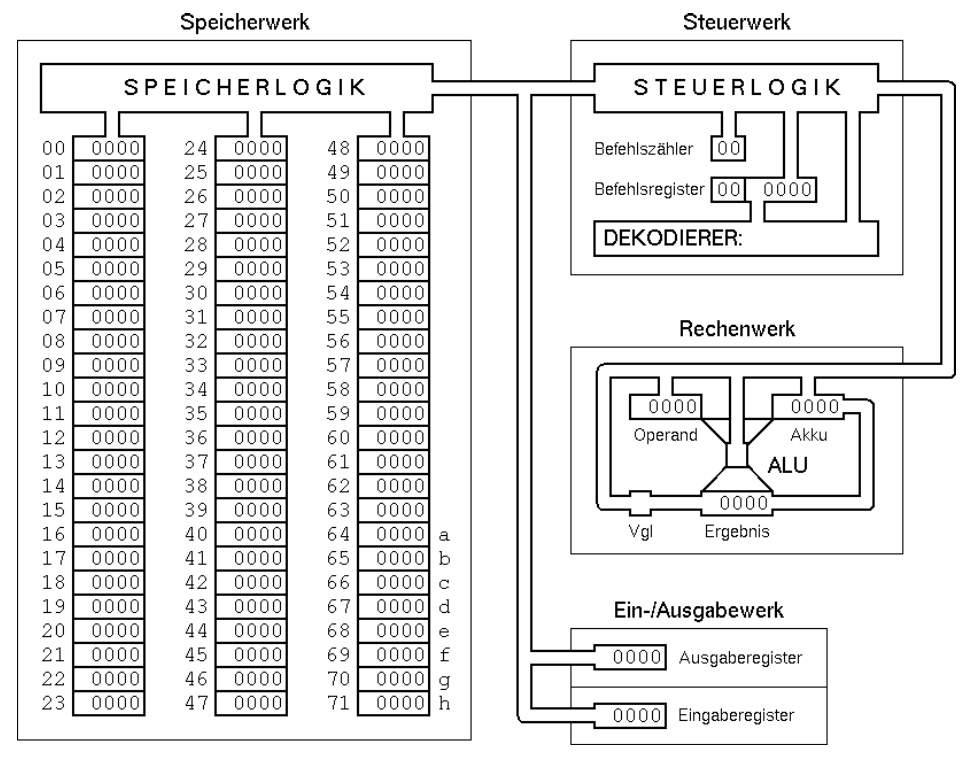
\includegraphics[width=0.8\textwidth]{mops}
\caption{Schematische Übersicht des MOPS}
\end{figure}
\vspace*{-2cm}
%
\Ueberschrift{Übungen}{task}
\begin{aufgaben}
\item \leicht Erklären Sie die fett gedruckten Begriffe mit maximal zwei prägnanten Sätzen.
\item \mittel Schreiben Sie ein Programm, das eine Zahl $n$ aus dem \textit{Eingaberegister} einliest und prüft, ob es sich um eine gerade Zahl handelt. Ist dies der Fall, soll eine $1$ in das \textit{Ausgaberegister} geschrieben werden, andernfalls eine $0$.
\item \schwer Schreiben Sie ein Programm, dass die Summe der ersten $n$ Zahlen berechnet. \textbf{Beispiel}: Die Summe der ersten $n=3$ Zahlen ist $1+2+\textbf{3}=6$. Dabei soll $n$ vom \textit{Eingaberegister} eingelesenen und das Ergebnis in das \textit{Ausgaberegister} geschrieben werden.
\end{aufgaben}
%
\newpage
\Quelle{Textquelle: Marco Haase}
\section*{MOPS-Befehlssatz}
Der Befehlssatz des MOPS-Assemblers umfasst insgesamt 15 Befehle. Die im folgenden aufgeführten Befehle beschreiben den eingebauten Befehlssatz. Dieser kann vom Benutzer bei Bedarf an die eigenen Vorstellungen angepasst werden: Es können für die einzelnen Befehle eigene mnemonische Codes festgelegt werden (max. 10 Zeichen, nur Buchstaben). Dazu verwendet man die optionale, aber mitgelieferte Datei mops.cfg. Wie man den MOPS mit einem eigenen Befehlssatz ausrüstet, wird in dieser Datei ebenfalls beschrieben. Der eingebaute Befehlssatz ist der folgende: 
%
\begin{table}[H]
\caption{Befehlssatz des Pseudo-Assemblers}
\renewcommand{\arraystretch}{1.5}
\begin{tabularx}{\textwidth}{|l|c|X|}
\hline 
\rule[-1ex]{0pt}{2.5ex} \textbf{Befehl} & \textbf{Code} & \textbf{Funktion} \\ 
\hline 
\rule[-1ex]{0pt}{2.5ex} ld \textit{adr} & 10 & \textbf{load}: Lade den Wert an der Adresse \textit{adr} in den Akku \\ 
\hline 
\rule[-1ex]{0pt}{2.5ex} ld \textit{val} & 11 & load: Lade den Wert \textit{val} in den Akku\\ 
\hline 
\rule[-1ex]{0pt}{2.5ex} st \textit{adr} & 12 & \textbf{store}: Speichere den Wert des Akku an der Adresse \textit{adr} \\ 
\hline 
\rule[-1ex]{0pt}{2.5ex} in \textit{adr} & 20 & \textbf{input}: Schreibe den Wert des Eingaberegisters an die Adresse \textit{adr} \\ 
\hline 
\rule[-1ex]{0pt}{2.5ex} out \textit{adr} & 22 & \textbf{output}: Schreibe den Wert an der Adresse \textit{adr} ins Ausgaberegister \\ 
\hline 
\rule[-1ex]{0pt}{2.5ex} out \textit{val} & 23 & output: Schreibe den Wert \textit{val} ins Ausgaberegister \\ 
\hline
\rule[-1ex]{0pt}{2.5ex} add \textit{adr} & 30 & \textbf{add}: Addiere den Wert an der Adresse \textit{adr} zum Akku \\ 
\hline 
\rule[-1ex]{0pt}{2.5ex} add \textit{val} & 31 & add: Addiere den Wert \textit{val} zum Akku \\ 
\hline 
\rule[-1ex]{0pt}{2.5ex} sub \textit{adr} & 32 & \textbf{subtract}: Subtrahiere den Wert an der Adresse \textit{adr} vom Akku \\ 
\hline 
\rule[-1ex]{0pt}{2.5ex} sub \textit{val} & 33 & subtract: Subtrahiere den Wert \textit{val} vom Akku \\ 
\hline 
\rule[-1ex]{0pt}{2.5ex} mul \textit{adr} & 34 & \textbf{multiply}: Multipliziere den Wert an der Adresse \textit{adr} mit dem Akku \\ 
\hline 
\rule[-1ex]{0pt}{2.5ex} mul \textit{val} & 35 & multiply: Multipliziere den Wert \textit{val} mit dem Akku \\ 
\hline 
\rule[-1ex]{0pt}{2.5ex} div \textit{adr} & 36 & \textbf{divide}: Dividiere den Akku durch den Wert an der Adresse \textit{adr} \\ 
\hline 
\rule[-1ex]{0pt}{2.5ex} div \textit{val} & 37 & divide: Dividiere den Akku durch den Wert \textit{val} (nur ganzzahliger Teil) \\ 
\hline 
\rule[-1ex]{0pt}{2.5ex} mod \textit{adr} & 38 &  \textbf{modulo}: Rest bei Division des Akku durch den Wert an der Adresse \textit{adr}\\ 
\hline 
\rule[-1ex]{0pt}{2.5ex} mod  \textit{val} & 39 & modulo: Rest bei Division des Akku durch den Wert \textit{val} \\ 
\hline 
\rule[-1ex]{0pt}{2.5ex} cmp \textit{adr} & 40 & \textbf{compare}: Vergleiche den Akkuinhalt mit dem Wert an der Adresse \textit{adr} \\ 
\hline 
\rule[-1ex]{0pt}{2.5ex} cmp  \textit{val} & 41 & compare: Vergleiche den Akkuinhalt mit dem Wert \textit{val} \\ 
\hline 
\rule[-1ex]{0pt}{2.5ex} jmp \textit{tar} & 50 & \textbf{jump}: Springe zum Zielpunkt \textit{tar} (Zeilennummer oder Marke) \\ 
\hline 
\rule[-1ex]{0pt}{2.5ex} jlt	\textit{tar} & 52 & \textbf{jump if less than}: Springe ..., wenn bei cmp der Akkuinhalt kleiner war \\ 
\hline 
\rule[-1ex]{0pt}{2.5ex} jeq \textit{tar} & 54 & \textbf{jump if equal}: Springe ..., wenn bei cmp der Akkuinhalt gleich war\\ 
\hline 
\rule[-1ex]{0pt}{2.5ex} jgt \textit{tar} & 56 & \textbf{jump if greater than}: Springe ..., wenn bei cmp der Akkuinhalt größer war \\ 
\hline 
\rule[-1ex]{0pt}{2.5ex} end & 60 & \textbf{end}: Beendet ein Programm \\ 
\hline 
\end{tabularx} 
\end{table}
\end{document}